USARSim is designed to communicate over 
%an American Standard Code for Information Interchange (ASCII) 
a TCP/IP socket with a computer hosting the controller of the robot. The robot is ``spawned'' into the simulated world running on the game server. 
A robot's configuration is controlled by an initialization file that resides on the simulation system's computer, comparable with the launch file from Gazebo. 
This file controls aspects such as sensor configuration, battery life, and simulated noise models. 
%Please see the USARSim wiki for more information on robot configuration~\cite{USARSimWeb}. 
 One socket connection is established per simulated robot, with both commands and sensor data being transmitted over the socket. An additional separate socket is established for high-volume sensors such as camera systems.

ROS stacks are designed to ``bottom out'' at a hardware abstraction layer that provides the interface 
to sensors and the motors of the robot; publishing and subscribing to the basic topics of the robot. 
For example, the mobility stack expects to be able to control a platform by writing commands to low-level topics that control items such as the velocity.
In addition, the mobility stack expects feedback from sensors, such as the movement detected by the inertia sensor. 
%These stacks may also place constraints or naming conventions on the topics.  
In order to close this low-level loop between ROS and USARSim, a USARSim package was created inside ROS\footnote{\url{http://sourceforge.net/projects/usarsimros/}}. This package contains a node called {\it RosSim} that publishes a ROS  transform tree \texttt{tf} and sensor messages, and also accepts platform and actuator motion commands. 
When run, it provides a mechanism for spawning a robot in USARSim, and then auto-discovering the robot's sensors, actuators, and drive configuration in order to provide the necessary ROS topics. 
 
 \begin{comment}
 \begin{table}[t!]
    \begin{center}
    \small{
    \begin{tabular}{ | l | l | p{4cm} |}
    \hline
    Parameter & Default & Definition \\ \hline
   robotType & P3AT & Type of robot to spawn. \\ \hline
   hostname & localhost & Name of host running USARSim. \\ \hline
   port & 3000 & TCP/IP Port on which USARSim listens. \\ \hline
   startPosition & Vehicle1 & Named location where robot should be spawned. This location is simulated world dependent. \\ \hline
   odomSensor & InsTest & Odometry sensor that should be used as the default sensor for feeding the {\it odom} topic of ROS.\\ \hline
    \end{tabular}
   }
    \caption{Parameters for USARSim ROS node.}
    \label{Table:USARSimNode}
    \end{center}
\end{table}
\end{comment}

\begin{figure}[t!]
\centering
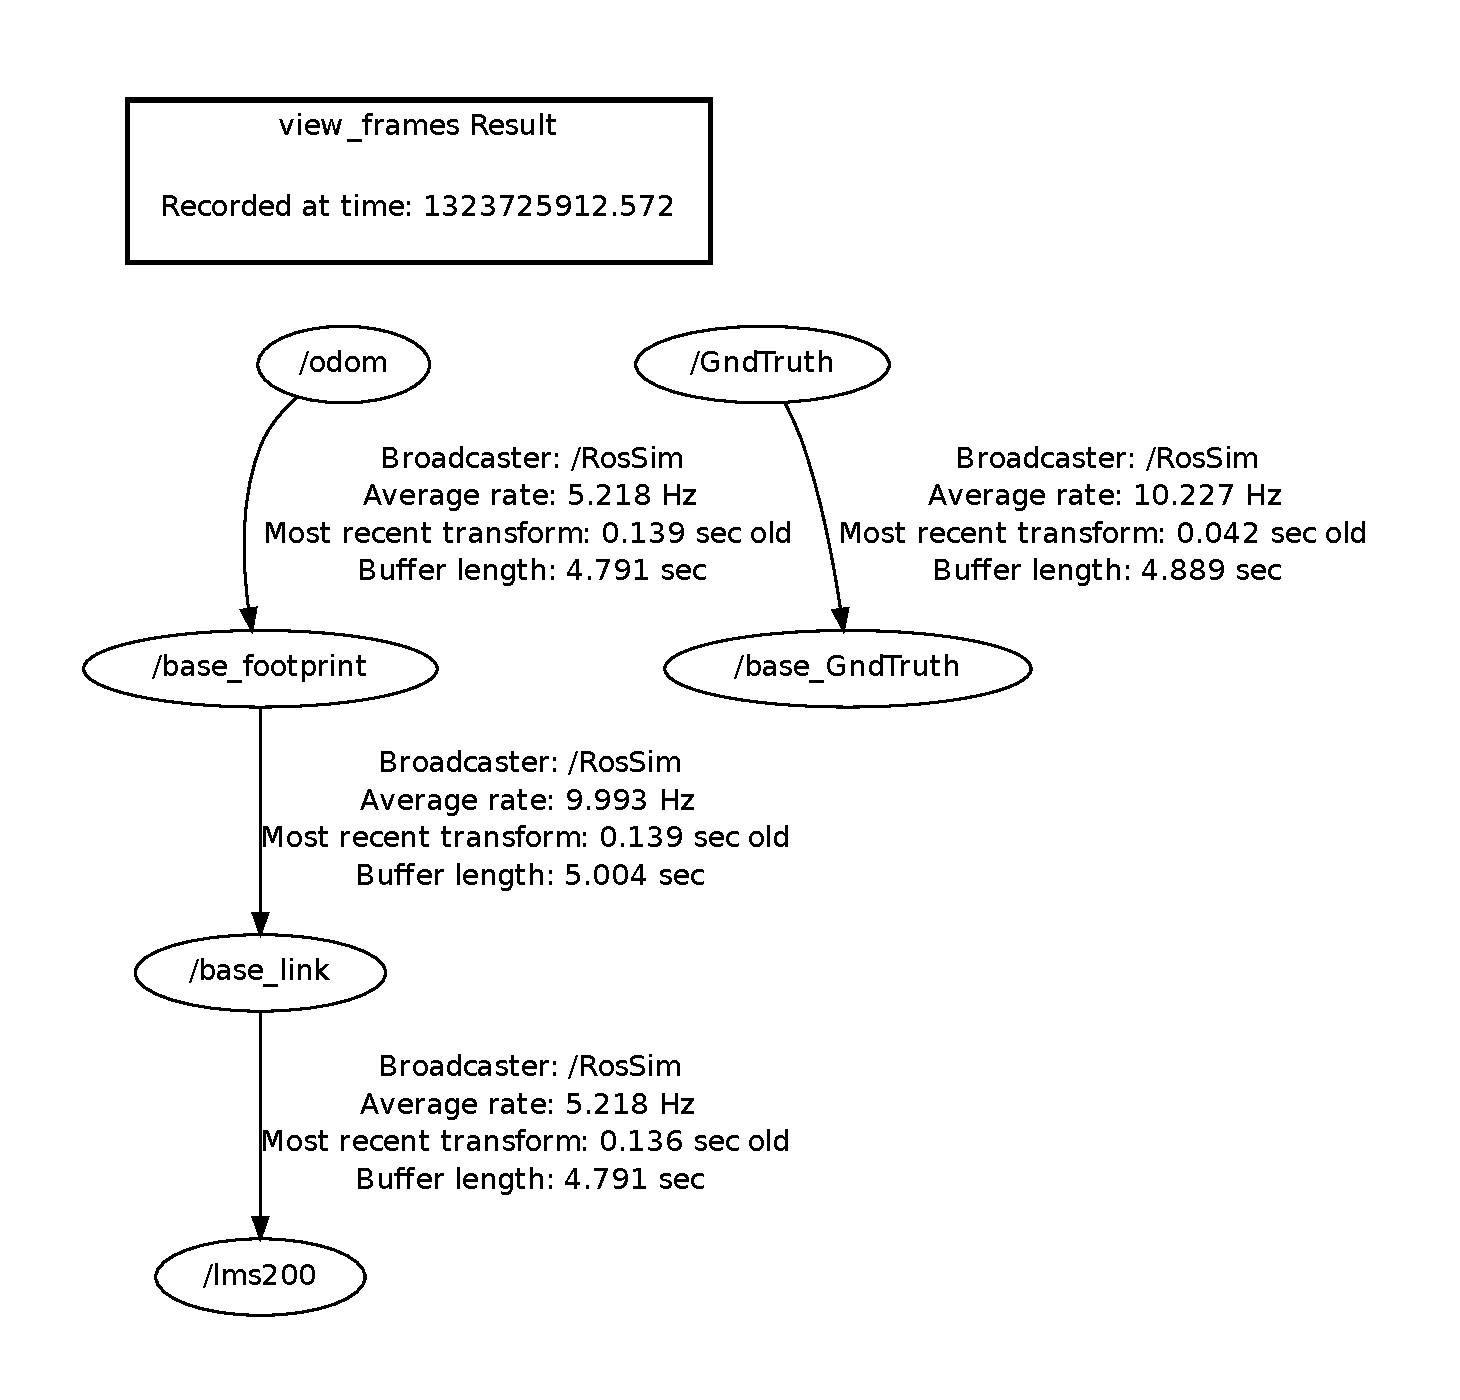
\includegraphics[width=8cm]{Figures/ROS/P3ATFrames.pdf}
\caption{Auto-generated \texttt{tf} transform tree for P3AT robot.}
\label{Fig:P3ATTransformTree}
\end{figure}

The {\it RosSim} node relies on several parameters for its configuration. These are 
%detailed in Table~\ref{Table:USARSimNode}, and provide information 
necessary for the creation of a robot in USARSim and a transform tree \texttt{tf} in ROS. 
A transform tree for the P3AT robot is shown in Figure~\ref{Fig:P3ATTransformTree}. 
This transform tree is built automatically from data obtained from the USARSim GEO and CONF messages. 
Since USARSim supports multiple sensors on a robot, 
%the {\it odomSensor} parameter is consulted to determine which sensor should be built into the tree. 
it should be specified which sensor should be preferred for an initial localization estimation (later updated in a SLAM algorithm).
That sensor's name is automatically changed to {\it odom}. The {\it base\_footprint}, representing the robot platform and the {\it base\_link} representing robot sensor mounting points are also automatically generated. 
%Additional  sensors are provided with each their own transform tree.

Vehicle movement commands into USARSim vary depending on the robot type. For example, skid-steered vehicles require left and right wheel velocities while Ackerman steered vehicles require steering angle and linear velocity. ROS provides a {\it cmd\_vel} topic that includes both linear and angular velocities. The {\it RosSim} node automatically converts these velocities into the appropriate commands and values for the USARSim simulator based on the robots steering type, wheelbase, and wheel separation. Vehicle speeds are also clamped to not exceed maximum velocities that are set in the simulation.
